\chapter{Técnicas de laboratório II: síntese e análise na prática}\label{ch:b2:lab-techniques-2}

Uma reação de Grignard fracassa numa segunda-feira de manhã: o balão tinha sido enxaguado mas não seco,
e as poucas gotas de água que restavam destruíram o reagente à medida que se formava. Refeita com
vidraria seca em estufa, sob nitrogênio, com o haleto adicionado gota a gota a um balão agitado e
resfriado, a mesma reação funciona. A química não mudou; a montagem, sim. Este capítulo trata da prática
que transforma uma reação no papel em um produto em um frasco: controlar a reação, manter fora o ar e a
água, fazer o \omterm{def:b2:lab-techniques-2:work-up}{tratamento}, purificar o produto e provar o que foi obtido.

\begin{omfigure}
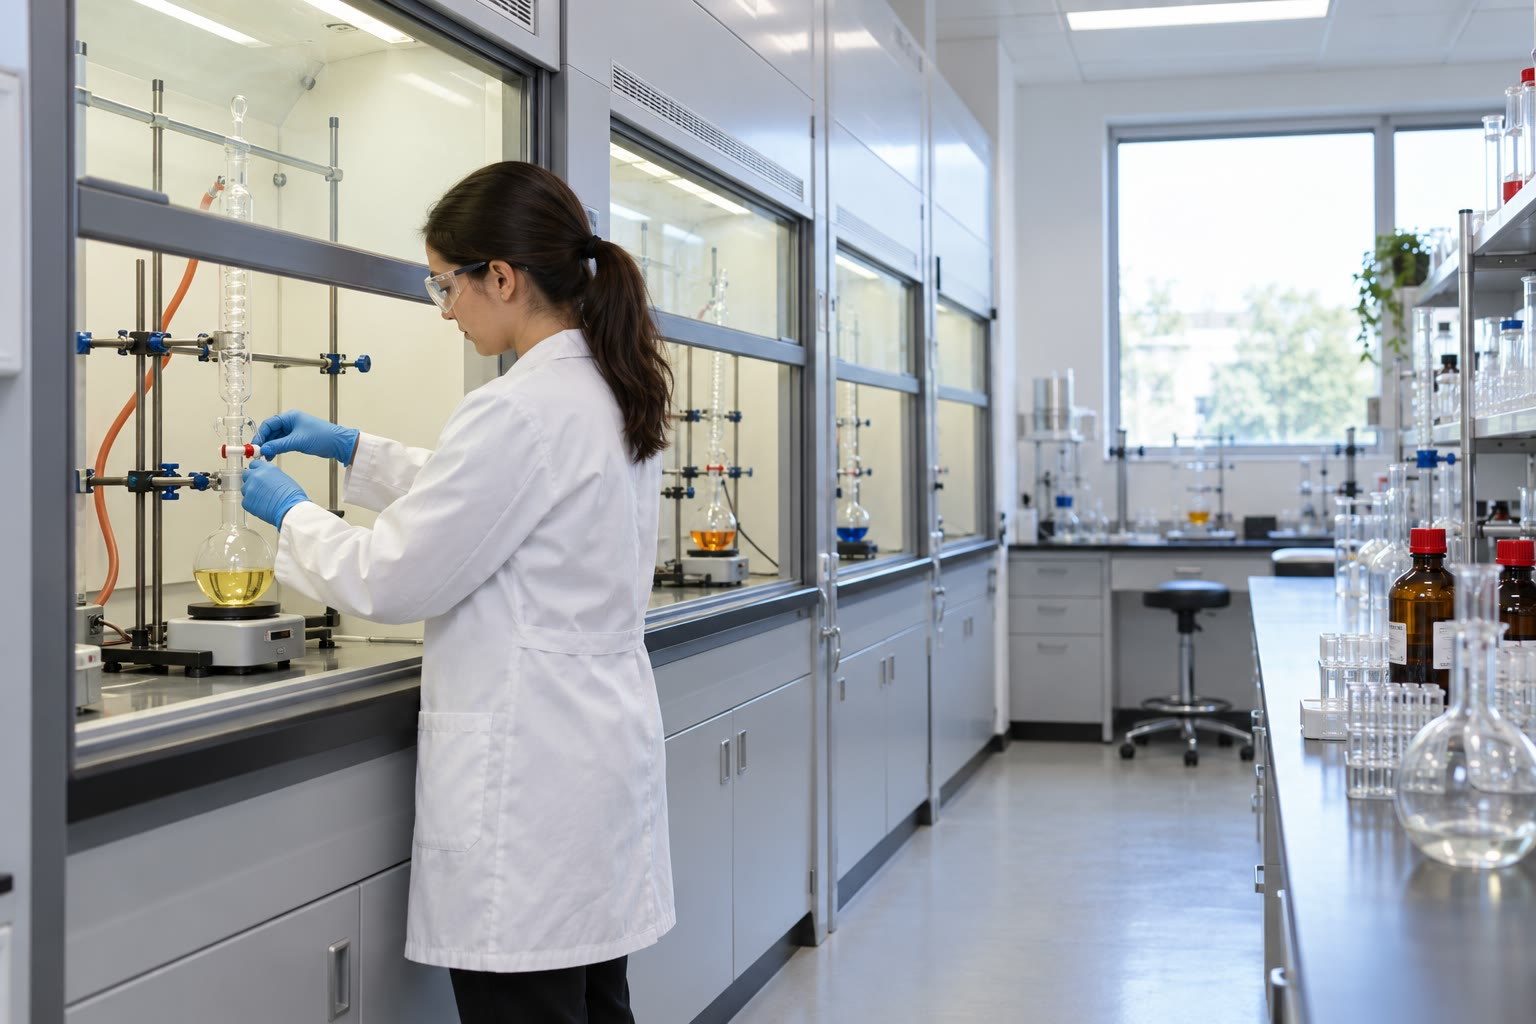
\includegraphics[width=0.56\linewidth]{images/book3/ai/b2-35-synthesis-lab.jpg}

{\small Um laboratório de síntese orgânica: reações conduzidas em capelas, balões presos em suportes
(ilustração).}
\end{omfigure}

\begin{recall}
O volume do 1.º ano: perigos e rótulos GHS, extração, recristalização, destilação, \omterm{def:b2:chromatography:principle}{cromatografia} em
camada delgada e $R_f$, ponto de fusão, reagentes de Grignard. \Cref{ch:b2:reaction-enthalpy}: \omterm{def:b2:reaction-enthalpy:reaction-quantity}{entalpia
de reação} e \omterm{def:b2:continuous-reactors:adiabatic-rise}{elevação adiabática de temperatura}. \Cref{ch:b2:chromatography},
\cref{ch:b2:structure-determination} e \cref{ch:b2:measurement-statistics}: a análise.
\end{recall}

\section{Conduzir uma reação sob controle}

Uma reação em um balão libera seu calor onde ocorre. O químico controla a temperatura com um banho
(gelo e água, gelo e sal, gelo-seco e acetona para as temperaturas mais baixas), com o refluxo de um
solvente em ebulição, que limita a temperatura a seu ponto de ebulição enquanto o condensador devolve o
vapor, e pela velocidade com que adiciona um reagente. Um termômetro interno, no líquido e não no
banho, mede o que importa.

\begin{proposition}[Acúmulo]\label{prop:b2:lab-techniques-2:accumulation}
Se um reagente é adicionado mais depressa do que reage, a quantidade que não reagiu $n_{\mathrm{acc}}$ se
acumula. Se ela reagir então de uma só vez, sem resfriamento, a temperatura da mistura de capacidade
térmica $C$ sobe de
\begin{equation*}
\Delta T_{\mathrm{ad}} = \frac{n_{\mathrm{acc}}\,|\Delta_rH|}{C}.
\end{equation*}
\end{proposition}

\begin{proof}
A reação de $n_{\mathrm{acc}}$ libera $n_{\mathrm{acc}}|\Delta_rH|$ a pressão constante
(\cref{ch:b2:reaction-enthalpy}); sem troca de calor, tudo isso aquece a mistura, como na \omterm{def:b2:reaction-enthalpy:flame-temperature}{temperatura
adiabática de chama} (\cref{def:b2:reaction-enthalpy:flame-temperature}): $C\Delta T =
n_{\mathrm{acc}}|\Delta_rH|$.
\end{proof}

O perigo é máximo quando uma reação demora a começar, como acontece muitas vezes com a formação dos
reagentes de Grignard: o haleto adicionado antes da iniciação se acumula, e quando a reação finalmente
começa ela dispara. A regra é adicionar uma pequena porção, ver a reação começar (aquecimento, turvação,
refluxo suave), e só então adicionar o resto na velocidade que o resfriamento consegue acompanhar.

\section{Condições anidras e atmosfera inerte}

\begin{definition}[Atmosfera inerte]\label{def:b2:lab-techniques-2:inert}
Uma reação é conduzida sob \emph{atmosfera inerte}\index{atmosfera inerte} quando o ar do aparelho foi
substituído por um gás não reativo, nitrogênio ou argônio, mantido em leve sobrepressão para que o ar não
possa entrar.
\end{definition}

Os reagentes organometálicos, os hidretos metálicos e muitos catalisadores reagem com a água e o
oxigênio. A vidraria é seca em estufa e montada ainda quente, ou flambada sob uma corrente de gás; os
solventes são comprados anidros ou secos sobre um reagente que reage com a água; os líquidos são
transferidos com seringas através de septos de borracha. O gás sai por um borbulhador de óleo, que
mostra o fluxo e impede o ar de refluir. A linha de Schlenk e a caixa de luvas, para os compostos mais
sensíveis, vêm no volume do 3.º ano.

\begin{omfigure}
\begin{tikzpicture}[lab/.style={font=\scriptsize, align=center}]
\fill[omDef!10] (-1.7,-0.3) rectangle (1.7,1.0);
\draw[om glass] (-1.7,1.2) -- (-1.7,-0.3) -- (1.7,-0.3) -- (1.7,1.2);
\foreach \x/\y in {-1.5/0.0,-1.45/0.55,1.3/0.05,1.3/0.6,-1.25/0.3,1.05/-0.15}{
  \draw[omDef!50, fill=white] (\x,\y) rectangle ++(0.18,0.18);}
\pic (f) at (0,0) {threeneck={0.35}{omThm!25}};
\pic[rotate=25] (d) at (f-l) {dropfunnel={0.5}{omMeth!20}};
\pic (c) at (f-c) {condenser};
\pic[rotate=-25] (t) at (0.0,0.42) {thermometer};
\pic (b) at (3.6,3.6) {bubbler};
\draw[thick, black!60] (0,6.25) -- (0,6.75) -- (3.25,6.75) -- (b-in);
\coordinate (dtop) at ($(f-l)+(-1.52,3.26)$);
\draw[thick, black!60] (dtop) -- ++(0,0.35) -- ++(-0.9,0) node[left, lab] {N$_2$};
\node[lab, anchor=north] at (0,-0.4) {banho de gelo};
\node[lab, anchor=east] at (-1.9,2.6) {funil de\\adição};
\node[lab, anchor=west] at (0.55,5.0) {condensador};
\node[lab, anchor=west] at (1.75,2.6) {termômetro\\(interno)};
\node[lab, anchor=north] at (3.6,3.45) {borbulhador (saída de gás)};
\end{tikzpicture}
\par\vspace{4pt}

{\small Uma reação sob nitrogênio (esquema). Balão de três bocas em um banho de gelo, com um termômetro
interno no líquido; o reagente é adicionado a partir de um funil de pressão equalizada pelo qual entra o
nitrogênio; o gás sai pelo condensador e por um borbulhador de óleo.}
\end{omfigure}

\begin{method}[Montar uma reação anidra sob nitrogênio]\label{met:b2:lab-techniques-2:anhydrous}
\begin{enumerate}
  \item Seque a vidraria em estufa e monte-a quente, engraxando ou encamisando as juntas; adapte um septo
        ou o funil de adição, o condensador e o borbulhador.
  \item Purgue com nitrogênio enquanto esfria; mantenha um fluxo lento (uma bolha a cada um ou dois
        segundos) durante todo o tempo.
  \item Adicione os sólidos antes da purga, os solventes anidros e os reagentes líquidos por seringa ou
        cânula através de um septo.
  \item Resfrie ou aqueça como previsto; comece a adição com uma pequena porção e verifique que a
        reação começa antes de continuar.
\end{enumerate}
\end{method}

\section{O tratamento}

\begin{definition}[Tratamento]\label{def:b2:lab-techniques-2:work-up}
O \emph{tratamento}\index{tratamento} de uma reação é a sequência de operações, após a reação, que
transforma a mistura reacional no produto bruto: extinção, extração e lavagem, secagem, filtração e
evaporação do solvente.
\end{definition}

\begin{definition}[Extração ácido--base]\label{def:b2:lab-techniques-2:acid-base-extraction}
Uma \emph{extração ácido--base}\index{extracao acido--base@extração ácido--base} separa compostos orgânicos ácidos, básicos e
neutros dissolvidos em um solvente orgânico lavando a solução com ácidos ou bases aquosos, que
convertem uma classe de compostos em íons que passam para a água.
\end{definition}

\begin{proposition}[Quem vai para onde]\label{prop:b2:lab-techniques-2:acid-base-extraction}
O hidrogenocarbonato de sódio aquoso (pH 8.3) extrai um ácido carboxílico ($\mathrm pK_a$ cerca de 4) mas
não um fenol ($\mathrm pK_a$ cerca de 10), que exige o hidróxido de sódio; o ácido clorídrico diluído
extrai uma amina cujo ácido conjugado tem $\mathrm pK_a$ de 4.6 ou mais; os compostos neutros ficam na
camada orgânica.
% ledger: ph:NaHCO3, pka:benzoic, pka:phenol, pka:anilinium
\end{proposition}

\begin{proof}
Uma espécie está sobretudo em sua forma básica quando $\mathrm{pH} > \mathrm pK_a$, e a mais de 99~\%
quando $\mathrm{pH} > \mathrm pK_a + 2$. A pH 8.3, o ácido benzoico (4.2) está a mais de 99~\% na forma
de benzoato, um íon que fica na água; o fenol (9.99) está a cerca de 2~\% na forma de fenóxido
($10^{8.3 - 10.0}$) e fica essencialmente na camada orgânica, para onde vai a forma neutra. No hidróxido
de sódio (pH acima de 12), o fenol é convertido em fenóxido. No ácido clorídrico diluído (pH cerca de 1),
a anilina (anilínio 4.6) está a mais de 99~\% na forma de anilínio. Cada íon, uma vez na água, é
recuperado levando o pH de volta no outro sentido, o que regenera o composto neutro, e extraindo-o de novo.
\end{proof}

\begin{omfigure}
\begin{tikzpicture}[x=1cm, y=1cm, st/.style={draw=black!70, rounded corners=2pt, fill=white,
  font=\scriptsize, align=center, inner sep=3pt, text width=3.0cm}, ar/.style={->, thick, black!70}]
\node[st, fill=omDef!10] (m) at (0,0) {ácido benzoico, fenol,\\anilina, naftaleno\\em etoxietano};
\node[st, fill=omThm!10] (a1) at (5.0,0) {fase aquosa: benzoato\\$\to$ HCl $\to$ ácido benzoico};
\node[st] (o1) at (0,-1.6) {fenol, anilina,\\naftaleno};
\node[st, fill=omThm!10] (a2) at (5.0,-1.6) {fase aquosa: fenóxido\\$\to$ HCl $\to$ fenol};
\node[st] (o2) at (0,-3.2) {anilina, naftaleno};
\node[st, fill=omThm!10] (a3) at (5.0,-3.2) {fase aquosa: anilínio\\$\to$ NaOH $\to$ anilina};
\node[st, fill=omMeth!10] (o3) at (0,-4.8) {naftaleno\\(secar, evaporar)};
\draw[ar] (m) -- node[above, font=\tiny] {NaHCO$_3$} (a1);
\draw[ar] (m) -- (o1); \draw[ar] (o1) -- node[above, font=\tiny] {NaOH} (a2);
\draw[ar] (o1) -- (o2); \draw[ar] (o2) -- node[above, font=\tiny] {HCl} (a3);
\draw[ar] (o2) -- (o3);
\pic at (8.6,-3.6) {sepfunnel={omDef!25}{omThm!20}};
\node[font=\scriptsize, align=center] at (8.6,-4.0) {funil de separação};
\end{tikzpicture}
\par\vspace{4pt}

{\small Separação ácido--base de quatro compostos (\cref{prop:b2:lab-techniques-2:acid-base-extraction}).
A camada orgânica (coluna da esquerda) perde uma classe a cada lavagem; cada extrato aquoso (à direita)
devolve seu composto quando o pH é invertido.}
\end{omfigure}

\begin{definition}[Agente secante]\label{def:b2:lab-techniques-2:drying-agent}
Um \emph{agente secante}\index{agente secante} é um sal anidro, como o sulfato de magnésio ou de sódio,
que fixa a água dissolvida em uma solução orgânica como água de hidratação e é depois removido por
filtração.
\end{definition}

\begin{method}[Do balão de reação ao produto bruto]\label{met:b2:lab-techniques-2:work-up}
\begin{enumerate}
  \item Extinga: destrua os reagentes reativos restantes com uma solução aquosa adequada, lentamente e
        com resfriamento.
  \item Extraia para um solvente orgânico; separe as camadas (verifique qual é qual adicionando uma gota
        de água); extraia de novo a camada aquosa.
  \item Lave as camadas orgânicas reunidas (ácido, base, depois salmoura, uma solução saturada de cloreto
        de sódio que remove a maior parte da água dissolvida).
  \item Seque com um \omterm{def:b2:lab-techniques-2:drying-agent}{agente secante} até que parte dele permaneça solta; filtre.
  \item Remova o solvente em um evaporador rotativo sob pressão reduzida; pese o produto bruto.
\end{enumerate}
\end{method}

\section{A purificação}

\begin{definition}[Cromatografia flash]\label{def:b2:lab-techniques-2:flash}
A \emph{cromatografia flash}\index{cromatografia flash} é uma \omterm{def:b2:chromatography:principle}{cromatografia} em coluna preparativa sobre sílica na
qual o eluente é empurrado através da coluna por uma leve pressão de gás, de modo que uma separação de
gramas de material leva minutos; o eluente é escolhido por \omterm{def:b2:chromatography:principle}{cromatografia} em camada delgada sobre a mesma
sílica.
\end{definition}

\begin{proposition}[Volumes de coluna]\label{prop:b2:lab-techniques-2:column-volumes}
Um composto que migra com $R_f$ em uma placa de CCD sai de uma coluna da mesma sílica e do mesmo eluente
após cerca de $1/R_f$ volumes de coluna de eluente.
\end{proposition}

\begin{proof}[Raciocínio]
Na placa, o composto percorre $R_f$ vezes a distância da frente do solvente: sua velocidade média é $R_f$
vezes a do eluente. Na coluna, a mesma partição dá a mesma razão de velocidades, de modo que o composto
precisa de $1/R_f$ vezes o volume de eluente que enche a coluna (o volume morto) para sair; na
linguagem do \cref{ch:b2:chromatography}, $R_f \approx 1/(1 + k)$. Um composto com $R_f = 0.25$
sai após cerca de quatro volumes de coluna, bem separado de um com 0.5 (dois volumes).
\end{proof}

\begin{omfigure}
\begin{tikzpicture}[lab/.style={font=\scriptsize, align=left, anchor=west}]
\pic (k) at (0,0) {chromcolumn={3.4}};
\node[lab] at (0.6,4.6) {eluente};
\node[lab] at (0.6,3.55) {areia};
\node[lab] at (0.6,2.2) {leito de sílica};
\foreach \i/\c in {0/white, 1/omThm!25, 2/omThm!25, 3/white, 4/omDef!25, 5/omDef!25, 6/white}{
  \pic at ({2.4+0.55*\i},-1.2) {testtube={0.45}{\c}};}
\node[font=\scriptsize] at (4.05,-1.6) {frações 1 a 7};
\pic at (7.6,-1.2) {tlcplate};
\foreach \j/\x in {2/7.15,3/7.45,5/7.75,6/8.05}{\node[font=\tiny] at (\x,-1.38) {\j};}
\fill[omThm] (7.45,0.95) circle (0.06); \fill[omThm] (7.15,0.95) circle (0.06);
\fill[omDef] (8.05,-0.05) circle (0.06); \fill[omDef] (7.75,-0.05) circle (0.06);
\node[font=\scriptsize, align=center] at (7.6,2.15) {CCD das\\frações};
\end{tikzpicture}
\par\vspace{4pt}

{\small \omterm{def:b2:lab-techniques-2:flash}{Cromatografia flash} (esquema). O produto bruto é depositado no topo da sílica e eluído; o
eluato é recolhido em frações; uma placa de CCD das frações mostra onde cada composto saiu (aqui o
composto rápido, apolar, nas frações 2--3, o mais lento em 5--6), e as frações puras são reunidas.}
\end{omfigure}

\begin{method}[Conduzir uma coluna flash]\label{met:b2:lab-techniques-2:flash}
\begin{enumerate}
  \item Escolha o eluente por CCD: o composto desejado com $R_f$ de cerca de 0.25--0.35, tão longe quanto
        possível das impurezas.
  \item Empacote a sílica (cerca de 30 a 100 vezes a massa de produto bruto) em suspensão ou a seco;
        acrescente uma camada de areia.
  \item Deposite o produto bruto no menor volume de solvente (ou adsorvido em um pouco de sílica).
  \item Elua sob leve pressão; recolha frações; verifique-as por CCD; reúna as puras e
        evapore.
\end{enumerate}
\end{method}

Os líquidos que se decompõem perto de seu ponto de ebulição são destilados sob pressão reduzida, onde
fervem a temperatura mais baixa.

\begin{definition}[Destilação sob pressão reduzida]\label{def:b2:lab-techniques-2:reduced-pressure}
Uma \emph{destilação sob pressão reduzida}\index{destilacao sob pressao reduzida@destilação sob pressão reduzida} é conduzida
em um aparelho ligado a uma bomba de vácuo através de um manômetro, a uma pressão em que o líquido ferve
a uma temperatura que ele suporta.
\end{definition}

\begin{proposition}[Ebulição sob pressão reduzida]\label{prop:b2:lab-techniques-2:reduced-pressure}
Com $T_b$ a temperatura de ebulição sob a pressão de referência $p^\circ$ e $\Delta_{\mathrm{vap}}H$
tratada como constante, a temperatura de ebulição sob a pressão $p$ é dada por
\begin{equation*}
\frac{1}{T} = \frac{1}{T_b} - \frac{R}{\Delta_{\mathrm{vap}}H}\ln\frac{p}{p^\circ}.
\end{equation*}
\end{proposition}

\begin{proof}
Um líquido ferve quando sua pressão de vapor iguala a pressão acima dele. A relação de Clausius--Clapeyron
da física, $\mathrm d\ln p/\mathrm dT = \Delta_{\mathrm{vap}}H/(RT^2)$ para um vapor ideal e um volume de
líquido desprezível, se integra entre $(T_b, p^\circ)$ e $(T, p)$ em $\ln(p/p^\circ) =
-(\Delta_{\mathrm{vap}}H/R)(1/T - 1/T_b)$; rearranjando, obtém-se o resultado.
\end{proof}

\begin{omfigure}
\begin{tikzpicture}
\begin{axis}[width=0.72\linewidth, height=5.2cm, xmode=log, xmin=5, xmax=1100, ymin=0, ymax=190,
  xlabel={pressão (\unit{mbar})}, ylabel={temperatura de ebulição (\unit{\degreeCelsius})},
  label style={font=\small}, tick label style={font=\scriptsize}, grid=major, grid style={black!10},
  legend style={font=\scriptsize, at={(0.02,0.98)}, anchor=north west}, legend cell align=left]
\addplot[omDef, thick] table[x=p, y=bromobenzene] {figdata/out/bachelor-2-vacuum-boiling.dat};
\addplot[omThm, thick] table[x=p, y=benzaldehyde] {figdata/out/bachelor-2-vacuum-boiling.dat};
\addplot[only marks, mark=o, mark size=2pt, omDef] coordinates {(7,27.75)};
\addplot[only marks, mark=o, mark size=2pt, omThm] coordinates {(13,61.85)};
\legend{bromobenzeno, benzaldeído, medido}
\end{axis}
\end{tikzpicture}

{\small Temperatura de ebulição em função da pressão (\cref{prop:b2:lab-techniques-2:reduced-pressure})
com as entalpias de vaporização e os pontos de ebulição do NIST WebBook. Os círculos são pontos de
ebulição medidos a 7 e \qty{13}{mbar}, não usados nas curvas: a equação simples fica a poucos kelvins.
Baixar a pressão de 1 bar a \qty{20}{mbar} baixa os pontos de ebulição em mais de
\qty{100}{K}.}
% figdata: bachelor-2/vacuum-boiling.py
% ledger: tb:bromobenzene, dvap:bromobenzene, tbp:bromobenzene.7mbar, tb:benzaldehyde, dvap:benzaldehyde, tbp:benzaldehyde.13mbar
\end{omfigure}

\section{Pureza e identidade}

Um produto é identificado comparando seus espectros e suas constantes físicas com os do composto esperado
(\cref{ch:b2:structure-determination}); sua pureza é medida separadamente, porque um produto pode ser o
composto certo e ainda assim conter vários por cento de outra coisa.

\begin{method}[Informar a pureza e o rendimento]\label{met:b2:lab-techniques-2:purity}
\begin{enumerate}
  \item Verifique a faixa de fusão de um sólido (estreita e próxima do valor da literatura para um
        composto puro) e sua CCD (uma só mancha em dois eluentes).
  \item Meça a pureza: porcentagem de área em CG ou CLAE (só uma estimativa, a menos que os \omterm{def:b2:chromatography:quantitative}{fatores de
        resposta} sejam conhecidos, \cref{ch:b2:chromatography}), ou RMN de prótons quantitativa,
        comparando uma integral do produto com uma de cada impureza, ou com um \omterm{def:b2:chromatography:quantitative}{padrão interno} pesado.
  \item Converta em fração mássica $w$ de produto no material isolado.
  \item Informe o rendimento corrigido pela pureza: $\rho = w\,m/(n_{\mathrm{lim}}M)$, onde $m$ é a
        massa isolada, $n_{\mathrm{lim}}$ a quantidade de reagente limitante e $M$ a massa molar.
\end{enumerate}
\end{method}

Para um produto opticamente ativo, a rotação específica acrescenta uma verificação de sua pureza
estereoquímica; o excesso enantiomérico e sua medida são tratados no volume do 3.º ano.

\begin{safety}{\ghs[5mm]{GHS02}\,\ghs[5mm]{GHS06}\,\ghs[5mm]{GHS07}\,\ghs[5mm]{GHS08}\,\ghs[5mm]{GHS09}}
O etoxietano e o oxolano são extremamente inflamáveis e formam peróxidos explosivos quando armazenados;
nenhuma chama no laboratório, teste os frascos antigos antes de destilar. O bromobenzeno é inflamável e
tóxico para a vida aquática; as aparas de magnésio são inflamáveis. A vidraria de vácuo é inspecionada
quanto a trincas em estrela e protegida.
% ledger: ghs:ether, ghs:THF, ghs:bromobenzene, ghs:Mg, ghs:MgSO4
\end{safety}

\section{Exercícios}

\begin{exercise}[$\star$]\label{exo:b2:lab-techniques-2:1}
Que banho você usaria para uma reação conduzida a cerca de \qty{0}{\degreeCelsius}, a cerca de
\qty{-15}{\degreeCelsius}, e a \qty{-78}{\degreeCelsius}?
\end{exercise}

\begin{exercise}[$\star$]\label{exo:b2:lab-techniques-2:2}
Uma extração usa diclorometano, mais denso que a água. Qual camada é a orgânica? Como verificar?
\end{exercise}

\begin{exercise}[$\star$]\label{exo:b2:lab-techniques-2:3}
Como saber que se adicionou sulfato de magnésio suficiente a uma solução em éter?
\end{exercise}

\begin{exercise}[$\star$]\label{exo:b2:lab-techniques-2:4}
Em hexano--acetato de etila 4\,:\,1, um produto tem $R_f = 0.65$ e uma impureza 0.75. O que você mudaria
para uma coluna, e em que sentido?
\end{exercise}

\begin{exercise}[$\star\star$]\label{exo:b2:lab-techniques-2:5}
Dê a ordem das lavagens que separam o ácido benzoico, o fenol, a anilina e o naftaleno de uma solução
em éter, justificando cada uma com um $\mathrm pK_a$, e como cada composto é recuperado.
\end{exercise}

\begin{exercise}[$\star\star$]\label{exo:b2:lab-techniques-2:6}
Estime as temperaturas de ebulição do bromobenzeno e do benzaldeído a \qty{20}{mbar}.
\end{exercise}

\begin{exercise}[$\star\star$]\label{exo:b2:lab-techniques-2:7}
Durante uma adição, \qty{0.050}{mol} de um reagente se acumularam sem reagir. Com $\Delta_rH =
\qty{-200}{kJ/mol}$ e uma capacidade térmica de \qty{400}{J/K} para a mistura (dados do exercício), que
elevação de temperatura poderia se seguir?
\end{exercise}

\begin{exercise}[$\star\star$]\label{exo:b2:lab-techniques-2:8}
Um cromatograma de CLAE mostra o produto a 96.0~\% da área total. Por que isso ainda não é uma pureza em
massa? Um espectro de prótons da mesma amostra mostra um singleto do produto (1H) de integral 1.00 e um
singleto de impureza (3H) de integral 0.12; produto \qty{200}{g/mol}, impureza \qty{100}{g/mol} (dados do
exercício). Calcule a fração mássica de produto.
\end{exercise}

\begin{exercise}[$\star\star$]\label{exo:b2:lab-techniques-2:9}
Obtêm-se \qty{4.10}{g} de um produto (\qty{164}{g/mol}) de pureza 95.0~\% (em massa) a partir de \qty{0.0300}{mol}
de reagente limitante. Calcule o rendimento, sem e com correção.
\end{exercise}

\begin{exercise}[$\star\star\star$]\label{exo:b2:lab-techniques-2:10}
Uma reação de Grignard deu benzeno e quase nenhum álcool após a adição do aldeído. Liste as causas
possíveis e como cada uma é evitada.
\end{exercise}

\begin{exercise}[$\star\star\star$]\label{exo:b2:lab-techniques-2:11}
Na ampliação de escala, \qty{1.00}{mol} de um haleto reage com $\Delta_rH = \qty{-270}{kJ/mol}$ em um
reator cujo resfriamento remove no máximo \qty{150}{W} (dados do exercício). Qual é o menor tempo de
adição seguro? O que acontece se a adição for mais rápida?
\end{exercise}

\begin{exercise}[$\star\star\star$]\label{exo:b2:lab-techniques-2:12}
Um sólido bruto de \qty{13.0}{g} poderia ser purificado por recristalização (uma etapa, 80~\% de
recuperação, pureza 99~\%) ou por \omterm{def:b2:lab-techniques-2:flash}{cromatografia flash} (95~\% de recuperação, pureza 99.5~\%, \qty{1.5}{L}
de solvente) (dados do exercício). Compare as duas vias.
\end{exercise}

\section{Problema: Um Grignard bem feito}

\begin{problem}[{Problema de fim de semana --- os perigos e uma montagem anidra, uma adição controlada e
o perigo do acúmulo, o tratamento, a purificação por cromatografia flash e um rendimento corrigido pela
pureza}]
\label{pb:b2:lab-techniques-2:1}
Dados do exercício. O brometo de fenilmagnésio é preparado a partir de \qty{15.7}{g} de bromobenzeno e
\qty{2.67}{g} de aparas de magnésio em etoxietano anidro, depois se adicionam \qty{9.55}{g} de
benzaldeído; o \omterm{def:b2:lab-techniques-2:work-up}{tratamento} com cloreto de amônio aquoso dá o difenilmetanol. Formação do reagente: $\Delta_rH =
\qty{-270}{kJ/mol}$; capacidade térmica da mistura \qty{170}{J/K}; início a \qty{20}{\degreeCelsius}. CCD
(hexano--acetato de etila 9\,:\,1): bifenila $R_f = 0.85$, difenilmetanol 0.25. Isolado após a coluna:
\qty{12.50}{g}. RMN de prótons desse material: o singleto \ce{CH(OH)} (1H) integra 1.00, a região
\omterm{def:b2:huckel:aromatic}{aromática} 10.90. Massas molares (\unit{g/mol}): bromobenzeno 157.01, benzaldeído 106.12, difenilmetanol
184.24, bifenila 154.21; Mg 24.305.
% ledger: ghs:ether, ghs:bromobenzene, ghs:Mg, ghs:benzaldehyde, ghs:NH4Cl, ghs:biphenyl, ghs:benzhydrol, tb:ether, aw:Mg, aw:C, aw:H, aw:Br, aw:O, nmr:biphenyl

\medskip
\noindent\textbf{Parte I --- Perigos e montagem.}
\begin{enumerate}
  \item Dê os principais perigos do etoxietano, do bromobenzeno e do magnésio.
  \item Escreva a reação do brometo de fenilmagnésio com a água, e explique a vidraria seca em estufa.
  \item Por que trabalhar sob nitrogênio?
  \item O que o borbulhador mostra, e o que ele impede?
  \item Por que o etoxietano é aqui um bom solvente?
  \item Calcule as quantidades de bromobenzeno e de magnésio. Qual está em excesso?
\end{enumerate}

\medskip
\noindent\textbf{Parte II --- Adição controlada.}
\begin{enumerate}[resume]
  \item Que calor libera a formação completa do reagente?
  \item Por que o bromobenzeno é adicionado gota a gota?
  \item A reação demora a começar, e 20~\% do bromobenzeno são adicionados antes que ela comece. Que
        calor pode então ser liberado de uma só vez?
  \item Calcule a \omterm{def:b2:continuous-reactors:adiabatic-rise}{elevação adiabática de temperatura}.
  \item Compare a temperatura final com o ponto de ebulição do etoxietano. O que acontece?
  \item Como a adição deve ser conduzida?
\end{enumerate}

\medskip
\noindent\textbf{Parte III --- Adição e \omterm{def:b2:lab-techniques-2:work-up}{tratamento}.}
\begin{enumerate}[resume]
  \item Escreva a reação com o benzaldeído e identifique o reagente limitante.
  \item Por que extinguir com cloreto de amônio e não com um ácido forte?
  \item Qual camada é a orgânica no funil de separação?
  \item Para que serve a lavagem com salmoura?
  \item Como a solução é seca, e como o solvente é removido?
  \item A bifenila é o principal subproduto. Como ela se forma, e o que a favorece?
\end{enumerate}

\medskip
\noindent\textbf{Parte IV --- Purificação e pureza.}
\begin{enumerate}[resume]
  \item Que composto sai primeiro da coluna?
  \item Após quantos volumes de coluna cada um sai?
  \item A partir das integrais de RMN, calcule a razão molar entre bifenila e álcool no material
        isolado.
  \item Calcule a fração mássica de difenilmetanol.
  \item Calcule a massa de difenilmetanol puro.
  \item Calcule a massa teórica.
  \item Calcule o rendimento sem correção pela pureza.
  \item Dê o rendimento corrigido pela pureza.
\end{enumerate}
\end{problem}
